\chapter{Chef Server}

The Chef Server acts as a hub for configuration data. The server stores cookbooks, the policies that are applied to nodes, and metadata that describes each registered node that is being managed by the chef-client. Nodes use the chef-client to ask the server for configuration details, such as recipes, templates, and file distributions. The chef-client then does as much of the configuration work as possible on the nodes themselves (and not on the server). This scalable approach distributes the configuration effort throughout the organization.

The diagram~\ref{fig:overview_chef_draft} shows the relationships between the various elements of Chef, including the nodes, the server, and the workstations. These elements work together to provide the chef-client the information and instruction that it needs so that it can do its job.

\begin{figure}[ht!]
  \center{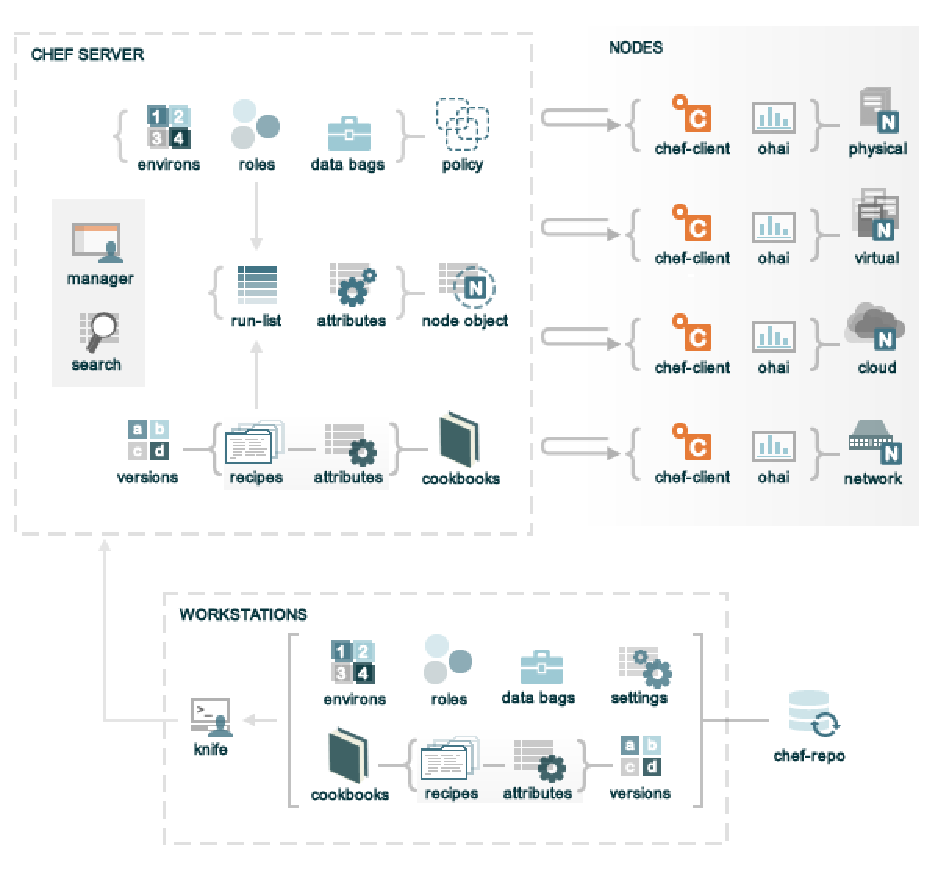
\includegraphics[width=1\textwidth]{overview_chef_draft}}
  \caption{Chef Infrastructure}
  \label{fig:overview_chef_draft}
\end{figure}